\documentclass[journal]{IEEEtran}
\usepackage[utf8]{inputenc}
\usepackage[T1]{fontenc}
\usepackage{amsmath,amssymb}
\usepackage{graphicx}
\usepackage{booktabs}
\usepackage{multirow}
\usepackage{tikz}
\usetikzlibrary{positioning,arrows.meta}
\usepackage[hidelinks]{hyperref}
\graphicspath{{figuras_en/}}
\hyphenpenalty=10000
\exhyphenpenalty=10000
\emergencystretch=2em

\begin{document}

\title{Atrial Fibrillation Detection in Intensive Care Electrocardiograms: Reproducing Handcrafted Feature Benchmarks and an Explainable Extension with Wavelet and Radon Transforms}

\author{Ricardo~A.~Acuña-Villogas%
\thanks{R. A. Acuña-Villogas is with the Department of Data Science, Universidad de Ingeniería y Tecnología (UTEC), Barranco, Lima, Peru (email: ricardo.acuna@utec.edu.pe). This work is the final project of the course EL5308 Biological Signals.}}

\markboth{EL5308 Biological Signals, Final Project, 2026}{Acuña-Villogas: Atrial Fibrillation Detection in ICU ECGs}

\maketitle

\noindent\textbf{Abstract:} Atrial fibrillation (AF) is the most frequent arrhythmia in the intensive care unit (ICU). Nassar et al. released the first public ICU AF dataset and benchmarks, without code. This work reproduces their feature based benchmark: 27 features per lead are extracted from 70\,203 PhysioNet/CinC 2021 recordings and 596 ICU recordings, and eight classifiers are trained under the two original configurations. The reproduced metrics deviate by at most 0.02 in AUROC and by 0.02 in mean F1, and confirm that logistic regression is the only model whose AUROC (0.97) survives the shift to ICU data. The study is extended with wavelet energies, Radon projections of recurrence plots, the atrial residual spectrum, a Cramér Rao analysis of heart rate estimation, and SHAP explanations. The kurtosis of the 45 degree Radon projection is the most discriminative of 172 features in both domains, the atrial dominant frequency lies between 5 and 8 Hz in AF, and heart rate estimation attains the Cramér Rao bound up to 20 ms of jitter. Under domain shift, the extended features raise the AUROC of CatBoost from 0.935 to 0.959. SHAP shows that the models rely first on absent P waves, a cue that weakens in the ICU.

\medskip
\noindent\textbf{Index Terms:} atrial fibrillation, electrocardiogram, intensive care unit, reproducibility, wavelet transform, Radon transform, recurrence plot, Cramér Rao bound, explainability, SHAP.

\section{Introduction}
\label{sec:intro}

Atrial fibrillation (AF) is the most common sustained arrhythmia and the most frequent one in critically ill patients, where new onset episodes are associated with longer stays, stroke, and higher mortality~\cite{kornej2020,moss2017,walkey2011}. Clinical guidelines define AF on the surface ECG by two signs: irregularly irregular RR intervals and the absence of distinct P waves, replaced by fibrillatory f waves~\cite{hindricks2021}. Continuous ECG monitoring in the intensive care unit (ICU) should make early detection straightforward, yet bedside monitors record only a few leads, the signals are contaminated by motion and electrode artifacts, and the false alarm burden of current arrhythmia algorithms is so high that it produces alarm fatigue~\cite{drew2014}. Reliable and interpretable AF detectors for this setting therefore remain an open need.

Most published AF detectors are trained and tested on ambulatory or diagnostic 12 lead ECGs, whose populations and acquisition conditions differ from those of the ICU~\cite{reyna2022}. Nassar et al.~\cite{nassar2025}, from the groups of P. Abolmaesumi and P. Mousavi, addressed this gap by releasing the Kingston ICU AF dataset, the first public set of ICU ECGs labeled for AF, and by benchmarking three families of methods on it: classical machine learning on handcrafted features, convolutional networks on signals and on time frequency images, and ECG foundation models. One of their observations is that classifiers trained on public data degrade when they are evaluated on ICU recordings, with the exception of linear models on handcrafted features. Their article, however, does not release source code, seeds, or several implementation details, so the extent to which its numbers can be recovered from the text alone is unknown. Reproducibility is a recognized weakness of machine learning research in medicine~\cite{pineau2021}, and a dataset paper is only as useful as the ability of others to rebuild its baselines.

This work rebuilds the feature based benchmark of~\cite{nassar2025} from its textual description and then asks a second question: whether classical signal analysis tools, namely the wavelet transform, the Radon transform, spectral estimation, and estimation theory, add information that the original heart rate variability features do not capture, and whether the resulting models reason in a clinically meaningful way. The main contributions are:
\begin{itemize}
\item An independent and resumable reimplementation of the feature based pipeline of~\cite{nassar2025}, including the labeling of 71\,148 PhysioNet/CinC 2021 recordings, that reproduces the published metrics of configurations 2 and 3 for eight classifiers within the sampling uncertainty of the test set.
\item An analysis of the sources of discrepancy in the absence of code, which separates unspecified choices (seeds, hyperparameters, missing value handling, library versions) from deliberate deviations.
\item Sixteen additional features per lead derived from the discrete wavelet transform, the Haar transform of the RR series, the Radon transform of delay embedded recurrence plots, and the spectrum of the atrial residual after QRST cancellation, evaluated with an ablation study with bootstrap confidence intervals.
\item A Cramér Rao analysis of heart rate estimation from 10 s windows, validated by Monte Carlo simulation, that bounds the information carried by the mean heart rate.
\item A SHAP based explanation of the models that links their decisions to the clinical definition of AF and identifies the P wave feature as the main casualty of the domain shift.
\end{itemize}

The rest of the paper is organized as follows. Section~\ref{sec:related} reviews related work. Section~\ref{sec:data} describes the datasets. Section~\ref{sec:methods} presents the reproduced pipeline and the proposed extensions. Section~\ref{sec:results} reports the reproduction, the extended analysis, and the explanations. Section~\ref{sec:discussion} discusses the findings and their limitations, and Section~\ref{sec:conclusion} concludes the paper.

\section{Related Work}
\label{sec:related}

\noindent\textbf{Feature based AF detection.} The classical approach summarizes the RR interval series with time domain, geometric, and nonlinear heart rate variability (HRV) measures, such as the standard deviation of successive differences, the proportion of successive differences above 50 ms (pNN50), Poincaré descriptors, and entropy, and feeds them to a conventional classifier~\cite{andreotti2017,jahan2022}. The PhysioNet/CinC 2017 Challenge showed that such features remain competitive with deep networks on short single lead recordings~\cite{clifford2017}. Toolboxes such as NeuroKit2~\cite{makowski2021} and R peak detectors derived from the Pan and Tompkins algorithm~\cite{pan1985,sleepecg} have made these pipelines standard.

\noindent\textbf{Deep learning and foundation models.} End to end networks reach cardiologist level performance on large ambulatory and 12 lead datasets~\cite{hannun2019,ribeiro2020}, and recent foundation models pretrained on millions of ECGs can be applied without retraining~\cite{mckeen2025,li2025}. In the ICU benchmark of~\cite{nassar2025}, zero shot foundation models obtained the best ranking metrics, while the best feature based model trained on public data obtained an F1 score of 0.84. The present work focuses on the feature based family because it is the one whose decisions can be traced to physiological quantities.

\noindent\textbf{Wavelets, recurrence, and Radon transforms.} The wavelet transform is a standard tool for ECG delineation and denoising, since its dyadic subbands align with the spectral content of the P, QRS, and T waves~\cite{addison2005,mallat2009}. Recurrence plots, built on the delay embedding theorem of Takens~\cite{takens1981}, visualize when a dynamical system returns to a previous state, and recurrence quantification analysis measures the length and density of their diagonal lines~\cite{marwan2007}. The Radon transform, the basis of computed tomography, integrates an image along lines of every orientation and is therefore a natural detector of oriented line structure~\cite{deans1983}. Combining both, the angular profile of the Radon transform of a recurrence plot summarizes how deterministic a rhythm is. In~\cite{nassar2025}, scaleograms and recurrence plots were used only as image inputs to convolutional networks.

\noindent\textbf{Atrial spectral analysis and explainability.} After cancellation of the ventricular activity, the spectrum of the surface ECG in AF shows a dominant atrial frequency between 4 and 9 Hz, and the concentration of power around that peak, the organization index, reflects the regularity of atrial activation~\cite{stridh2001,bollmann2006}. SHAP values~\cite{lundberg2017}, computed exactly for tree ensembles by TreeSHAP~\cite{lundberg2020}, have become the most common way to attribute the output of tabular clinical models to their inputs.

\section{Data}
\label{sec:data}

\noindent\textbf{Kingston ICU AF dataset.} The dataset of~\cite{nassar2025} contains 596 ECGs of 10 s from distinct ICU patients, recorded at 240 Hz with leads I, II, III, and a V1 equivalent, and labeled by clinicians as sinus rhythm (497) or AF and atrial flutter (99). The metadata include the stratified split into two halves used in the original study: 298 recordings for training (50 AF) and 298 for testing (49 AF). All metrics in this work are computed on the same test half.

\noindent\textbf{PhysioNet/CinC 2021.} The public training set of the 2021 Challenge~\cite{reyna2021,goldberger2000} contains 12 lead ECGs from several institutions. Chapman, Ningbo, and PTB XL were obtained from the open PhysioNet mirror on AWS, and CPSC 2018 and Georgia from physionet.org. Following~\cite{nassar2025}, SNOMED codes for sinus rhythm, sinus bradycardia, sinus tachycardia, and sinus arrhythmia define the negative class, and codes for AF and atrial flutter define the positive class. Recordings with both classes or with labels absent from the ICU set (pacemaker, bigeminy, trigeminy, ventricular arrhythmias, and other tachycardias or bradycardias) are removed, and leads I, II, III, and V1 are kept. Table~\ref{tab:data} compares the result with the counts reported in the original article.

\begin{table}[t]
\centering
\caption{Public recordings after labeling, compared with Table II of~\cite{nassar2025}.}
\label{tab:data}
\begin{tabular}{lrrrr}
\toprule
& \multicolumn{2}{c}{Recordings} & \multicolumn{2}{c}{AF prevalence} \\
Source & Ours & \cite{nassar2025} & Ours & \cite{nassar2025} \\
\midrule
Chapman and Ningbo & 42\,316 & 41\,331 & 0.21 & 0.22 \\
CPSC 2018 and Extra & 2\,701 & 2\,687 & 0.53 & 0.53 \\
Georgia & 5\,610 & 5\,623 & 0.12 & 0.12 \\
PTB and PTB XL & 20\,521 & 20\,722 & 0.08 & 0.07 \\
\midrule
Total & 71\,148 & 70\,363 & 0.18 & 0.18 \\
\bottomrule
\end{tabular}
\end{table}

After feature extraction, 883 public recordings were discarded because one of the four leads was flat and 43 because a lead had three R peaks or fewer, which leaves 70\,203 recordings for training, 0.2\% fewer than in~\cite{nassar2025}. All 596 ICU recordings produced valid features. Fig.~\ref{fig:ecg} shows two examples after preprocessing.

\begin{figure}[t]
\centering
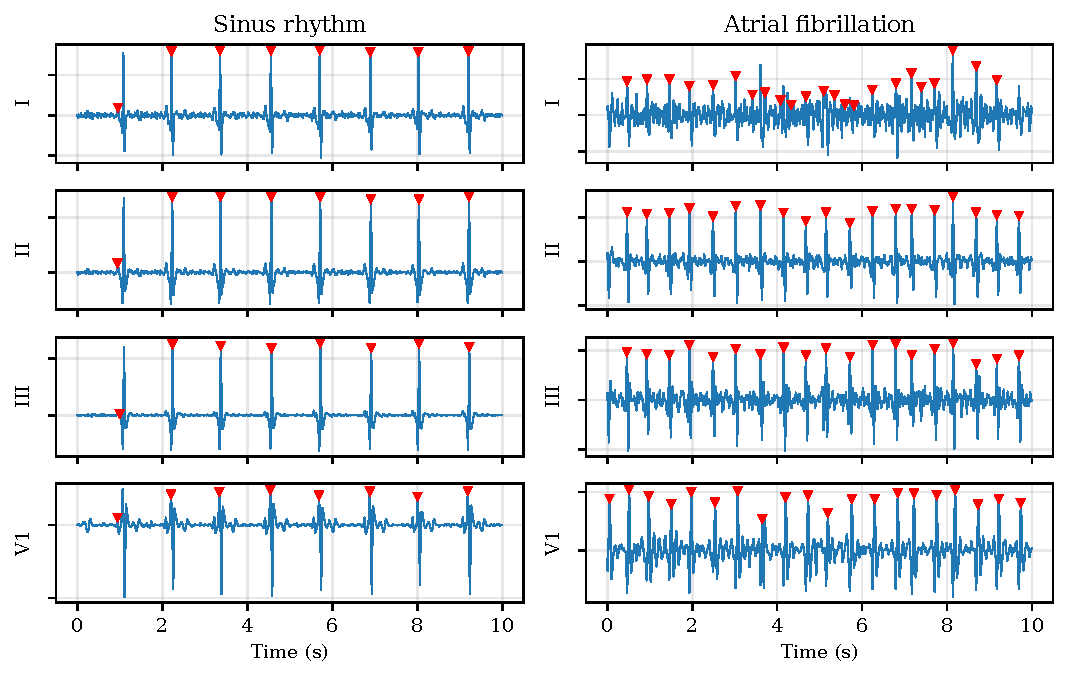
\includegraphics[width=\columnwidth]{ecg_examples.pdf}
\caption{Four lead ECGs after band pass filtering and resampling to 240 Hz, with the detected R peaks. In sinus rhythm (left) the RR intervals are nearly constant and a P wave precedes each QRS complex; in AF (right) the intervals are irregular and the baseline oscillates without P waves.}
\label{fig:ecg}
\end{figure}

\section{Methods}
\label{sec:methods}

Fig.~\ref{fig:pipeline} summarizes the pipeline. The reproduced part follows~\cite{nassar2025}; the extension adds new feature groups and analyses without altering the reproduced steps.

\begin{figure}[t]
\centering
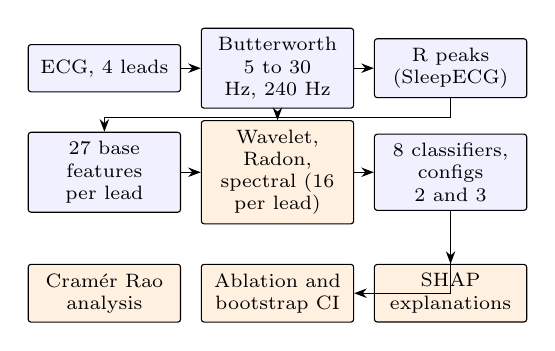
\begin{tikzpicture}[node distance=2.5mm, every node/.style={font=\scriptsize, align=center},
 caja/.style={draw, rounded corners=1pt, minimum height=6mm, text width=17mm, fill=blue!6},
 ext/.style={draw, rounded corners=1pt, minimum height=6mm, text width=17mm, fill=orange!12},
 flecha/.style={-{Stealth[length=1.6mm]}}]
\node[caja] (a) {ECG, 4 leads};
\node[caja, right=of a] (b) {Butterworth 5 to 30 Hz, 240 Hz};
\node[caja, right=of b] (c) {R peaks (SleepECG)};
\node[caja, below=5mm of a] (d) {27 base features per lead};
\node[ext, right=of d] (e) {Wavelet, Radon, spectral (16 per lead)};
\node[caja, right=of e] (f) {8 classifiers, configs 2 and 3};
\node[ext, below=5mm of e] (g) {Ablation and bootstrap CI};
\node[ext, right=of g] (h) {SHAP explanations};
\node[ext, left=of g] (i) {Cramér Rao analysis};
\draw[flecha] (a) -- (b); \draw[flecha] (b) -- (c);
\draw[flecha] (c.south) |- ++(0,-2.5mm) -| (d.north);
\draw[flecha] (c.south) |- ++(0,-2.5mm) -| (e.north);
\draw[flecha] (d) -- (e); \draw[flecha] (e) -- (f);
\draw[flecha] (f) |- (g); \draw[flecha] (f) -- (h);
\end{tikzpicture}
\caption{Pipeline of this work. Blue blocks reproduce~\cite{nassar2025}; orange blocks are the extension proposed here.}
\label{fig:pipeline}
\end{figure}

\subsection{Reproduced Pipeline}

\noindent\textbf{Preprocessing.} Each lead is filtered with a second order Butterworth band pass filter between 5 and 30 Hz applied forward and backward (zero phase), and public signals are resampled from 500 Hz to 240 Hz with a polyphase filter. Only the first 10 s of each recording are used. The forward and backward application squares the magnitude response, which doubles the stopband attenuation in decibels and removes the phase delay, so that R peak locations are preserved.

\noindent\textbf{Base features.} R peaks are detected with SleepECG~\cite{sleepecg}, and NeuroKit2~\cite{makowski2021} computes 27 features per lead: signal quality, heart rate, nine statistics of the RR intervals, SDSD, pNN20, pNN50, the HRV triangular index, eleven Poincaré descriptors (SD1, SD2, ellipse area, and the contributions of accelerations and decelerations), the percentage of inflection points, Shannon entropy, and the mean P wave amplitude. Concatenating the four leads yields 108 columns.

\noindent\textbf{Classifiers.} The eight models of~\cite{nassar2025} are used with library defaults: k nearest neighbours (KNN), a multilayer perceptron (MLP), a support vector machine (SVM) with RBF kernel, logistic regression (LR), and four ensembles of 1000 trees: random forest (RF), LightGBM~\cite{ke2017}, XGBoost~\cite{chen2016}, and CatBoost~\cite{prokhorenkova2018}. Features are imputed with the training median and min max scaled, and the decision threshold is 0.5. In configuration 2 the models are trained on the ICU training half; in configuration 3 they are trained on the public data. Both are tested on the ICU test half.

\noindent\textbf{Unspecified choices and deviations.} The original article does not release code or seeds and does not specify the number of neighbours, the MLP architecture, the SVM kernel, the handling of missing feature values, the NeuroKit2 methods for signal quality and P wave delineation, or the library versions. Library defaults, a fixed seed, and median imputation were adopted for these choices. The only deliberate deviation is that the SVM of configuration 3 is trained on a stratified subsample of 20\,000 recordings, because the cost of kernel SVM training grows roughly with the square of the number of samples.

\subsection{Wavelet Features}

The continuous wavelet transform with a Morlet mother wavelet provides scaleograms for visual inspection. For features, the discrete wavelet transform with the Daubechies 4 wavelet decomposes each lead at 240 Hz into five levels, whose approximate bands are A5 (0 to 3.75 Hz), D5 (3.75 to 7.5 Hz), D4 (7.5 to 15 Hz), D3 (15 to 30 Hz), D2, and D1. The relative energy of each subband and the wavelet entropy give seven features. The Haar transform is also applied to the RR interval series: the relative energy of its level 1 and level 2 details measures how much consecutive intervals differ, which is the defining property of AF.

\subsection{Radon Transform of Recurrence Plots}

Let $x_n$ be the filtered lead. With delay embedding $\mathbf{v}_i = (x_i, x_{i+\tau}, x_{i+2\tau})$, $\tau = 2$, on 256 samples, the recurrence plot is
\begin{equation}
RP_{ij} = \Theta\left(\varepsilon - \lVert \mathbf{v}_i - \mathbf{v}_j \rVert\right),
\end{equation}
where $\Theta$ is the Heaviside function and $\varepsilon$ is chosen for a recurrence rate of 10\%. A periodic signal produces long lines parallel to the main diagonal, at distances equal to the period. The Radon transform of the centered plot,
\begin{equation}
\mathcal{R}f(\rho, \theta) = \iint f(x, y)\,\delta(x\cos\theta + y\sin\theta - \rho)\,dx\,dy,
\end{equation}
integrates it along lines of angle $\theta$. At $\theta = 45^\circ$ each diagonal line collapses into a single value of $\rho$, so a regular rhythm produces a projection with several strong peaks, whereas in AF only the main diagonal survives. Four features are extracted: the variance of the $45^\circ$ projection, its ratio to the mean variance over all angles, the angle of maximum variance, and the kurtosis of the $45^\circ$ projection.

\subsection{Spectrum of the Atrial Residual}

Ventricular activity is cancelled by subtracting from each beat an average QRST template aligned on the R peaks~\cite{stridh2001}. The power spectral density of the residual is estimated with Welch's method, and three features are computed in the 3 to 12 Hz band: the dominant frequency, the organization index (power within 0.5 Hz of the dominant frequency divided by the band power), and the normalized spectral entropy~\cite{bollmann2006}. With the wavelet, Haar, and Radon groups, the extension adds 16 features per lead, for a total of 172 columns.

\subsection{Cramér Rao Bound for Heart Rate}

In regular rhythm the R peak times follow the linear model
\begin{equation}
t_k = t_0 + kT + w_k, \quad k = 0, \dots, K-1, \quad w_k \sim \mathcal{N}(0, \sigma^2),
\end{equation}
where $T$ is the cardiac period and $w_k$ combines physiological jitter and detection error. The Fisher information matrix of $(t_0, T)$ is
\begin{equation}
\mathbf{I}(t_0, T) = \frac{1}{\sigma^2}\begin{bmatrix} K & \sum_k k \\ \sum_k k & \sum_k k^2 \end{bmatrix},
\end{equation}
and its inverse gives $\mathrm{var}(\hat T) \geq 12\sigma^2 / [K(K^2-1)]$~\cite{kay1993}. Since the heart rate is $HR = 60/T$, the transformation of parameters yields
\begin{equation}
\mathrm{var}(\widehat{HR}) \geq \left(\frac{60}{T^2}\right)^2 \frac{12\,\sigma^2}{K(K^2-1)}.
\label{eq:crlb}
\end{equation}
For this linear Gaussian model the least squares line fit is efficient. To verify the bound under realistic detection, synthetic ECGs of 10 s at 240 Hz and 73 beats per minute are built as sums of Gaussian P, Q, R, S, and T waves. Each beat receives an independent Gaussian displacement with standard deviation between 1 and 40 ms, white noise at 20 dB SNR is added, R peaks are detected with the same filter and detector, and the line is fitted; this is repeated 400 times per jitter level. The bound uses $\sigma^2$ equal to the jitter variance plus the quantization variance $\Delta^2/12$, with $\Delta = 1/240$ s.

\subsection{Evaluation and Explainability}

The metrics are AUROC, AUPRC, F1 score, and the Matthews correlation coefficient (MCC). The ablation compares five feature sets (base, base with wavelet, base with Radon, base with spectral, and all) for LR, KNN, and CatBoost, with 95\% confidence intervals from 1000 bootstrap resamples of the test set~\cite{efron1993}; differences between sets are assessed with paired bootstrap intervals of the difference. The univariate discriminative power of each feature is measured by its AUROC, taken as $\max(A, 1-A)$. SHAP values are computed with TreeSHAP~\cite{lundberg2020} for the CatBoost model of configuration 3 with all features, on the ICU test set.

\noindent\textbf{Implementation.} Feature extraction runs in parallel with checkpoints every 200 recordings, and every trained model stores its test probabilities, so the full pipeline can be interrupted and resumed. Extracting features from the public data took about 2.5 h on seven processes of a laptop CPU, and training all models took 7 min.

\section{Results}
\label{sec:results}

\subsection{Reproduction}

Table~\ref{tab:repro} compares the reproduced metrics with Tables S2 and S3 of~\cite{nassar2025}. Across the 16 model and configuration pairs, the largest AUROC deviation is 0.02 and the mean absolute F1 deviation is 0.02. With 49 positive cases in the test set, a single additional or missing true positive changes F1 by about 0.01 to 0.02, so the observed deviations are of the order of one or two classified cases. The largest deviation, the F1 of the MLP in configuration 2 (0.78 against 0.83), corresponds to the model most sensitive to initialization and trained on only 298 samples.

\begin{table*}[t]
\centering
\caption{Published (Pub.) and reproduced (Rep.) metrics on the Kingston ICU test set ($n = 298$, 49 AF). Configuration 2 trains on the ICU training half and configuration 3 on PhysioNet/CinC 2021.}
\label{tab:repro}
\begin{tabular}{l cc cc cc cc c cc cc cc cc}
\toprule
& \multicolumn{8}{c}{Configuration 2} && \multicolumn{8}{c}{Configuration 3} \\
\cmidrule{2-9}\cmidrule{11-18}
& \multicolumn{2}{c}{AUROC} & \multicolumn{2}{c}{AUPRC} & \multicolumn{2}{c}{F1} & \multicolumn{2}{c}{MCC} && \multicolumn{2}{c}{AUROC} & \multicolumn{2}{c}{AUPRC} & \multicolumn{2}{c}{F1} & \multicolumn{2}{c}{MCC} \\
Model & Pub. & Rep. & Pub. & Rep. & Pub. & Rep. & Pub. & Rep. && Pub. & Rep. & Pub. & Rep. & Pub. & Rep. & Pub. & Rep. \\
\midrule
KNN       & .95 & .94 & .82 & .80 & \textbf{.83} & .82 & .79 & .79 &  & .90 & .91 & .74 & .76 & .81 & .77 & .77 & .72 \\
MLP      & .96 & .94 & .91 & .88 & \textbf{.83} & .78 & \textbf{.80} & .74 &  & .93 & .92 & .82 & .83 & .79 & .80 & .76 & .77 \\
SVM      & \textbf{.97} & .96 & .89 & .89 & .81 & .81 & .77 & .78 &  & .93 & .92 & .87 & .86 & \textbf{.84} & \textbf{.82} & \textbf{.81} & \textbf{.79} \\
LR       & \textbf{.97} & \textbf{.97} & .88 & .89 & .80 & .79 & .76 & .75 &  & \textbf{.97} & \textbf{.97} & \textbf{.88} & \textbf{.90} & .81 & \textbf{.82} & .77 & \textbf{.79} \\
RF       & .96 & .96 & .89 & .89 & .78 & .79 & .75 & .76 &  & .93 & .93 & .86 & .87 & .76 & .78 & .72 & .75 \\
LightGBM & \textbf{.97} & \textbf{.97} & \textbf{.92} & \textbf{.91} & .81 & .83 & .77 & .80 &  & .93 & .93 & .86 & .86 & .78 & \textbf{.82} & .74 & \textbf{.79} \\
XGBoost  & \textbf{.97} & .96 & .90 & .89 & .82 & \textbf{.84} & .79 & \textbf{.81} &  & .94 & .93 & .86 & .86 & .78 & .78 & .74 & .73 \\
CatBoost & \textbf{.97} & \textbf{.97} & .91 & \textbf{.91} & \textbf{.83} & \textbf{.84} & .79 & .80 &  & .94 & .93 & .87 & .85 & .77 & .76 & .72 & .71 \\
\bottomrule
\end{tabular}
\end{table*}

The qualitative conclusions of the original article are also recovered. Within the ICU (configuration 2), all models reach an AUROC between 0.94 and 0.97 and no model dominates the others in F1. Under domain shift (configuration 3), LR keeps its AUROC of 0.97, whereas the tree ensembles, the MLP, and KNN fall to between 0.91 and 0.93. Fig.~\ref{fig:roc} shows that the curves of all models rise almost vertically: about 80\% of AF episodes are detected with very few false alarms, and the models differ only in the remaining hard cases, where the precision of every model except LR collapses beyond a recall of 0.8.

\begin{figure}[t]
\centering
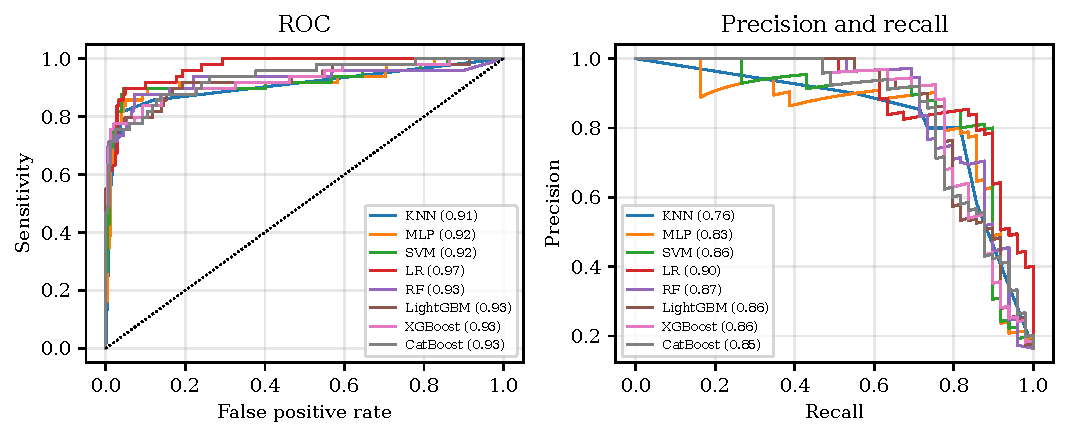
\includegraphics[width=\columnwidth]{roc_pr_conf3.pdf}
\caption{ROC and precision recall curves of the eight reproduced models in configuration 3 (public training, ICU test). The area under each curve is given in parentheses.}
\label{fig:roc}
\end{figure}

\subsection{Wavelet Analysis}

The scaleograms of Fig.~\ref{fig:scal} display the two signatures of AF in a single map. In sinus rhythm the QRS complexes form equally spaced columns of energy; in AF the columns are irregularly spaced and the band below 8 Hz keeps energy between beats, which corresponds to the f waves. As features, however, the discrete wavelet energies of the filtered signal separate the classes poorly (Fig.~\ref{fig:wav} and Table~\ref{tab:univ}). The 5 to 30 Hz filter of the reproduced pipeline removes most of the f wave band, and the remaining energy is dominated by the QRS complex in D4 and D3. The Haar detail energy of the RR series shifts towards higher values in AF, as expected from the beat to beat irregularity, but its normalization by the total energy of the series discards the absolute scale of variability, and it is weaker than pNN50 on its own.

\begin{figure}[t]
\centering
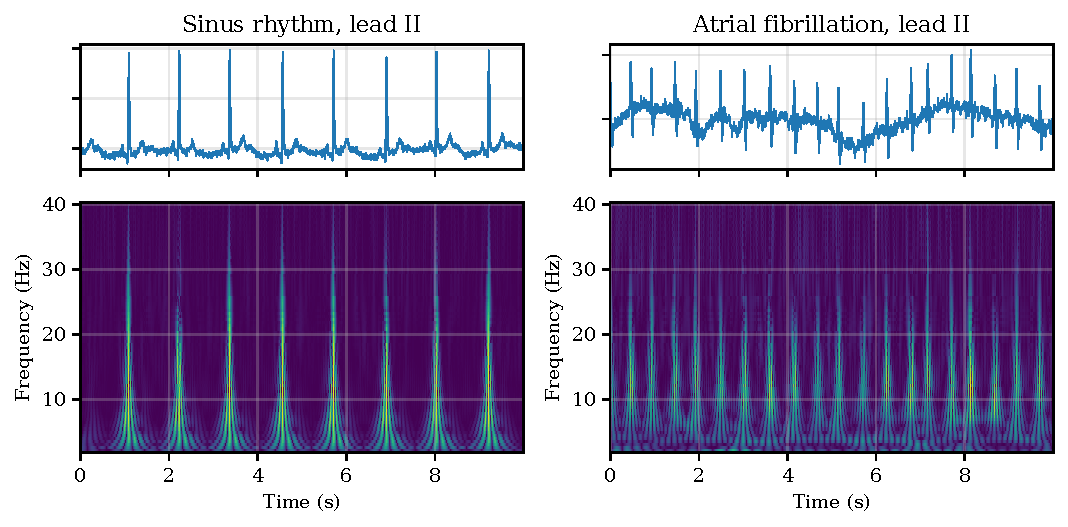
\includegraphics[width=\columnwidth]{scalograms.pdf}
\caption{Lead II and its Morlet scaleogram in sinus rhythm and in AF.}
\label{fig:scal}
\end{figure}

\begin{figure}[t]
\centering
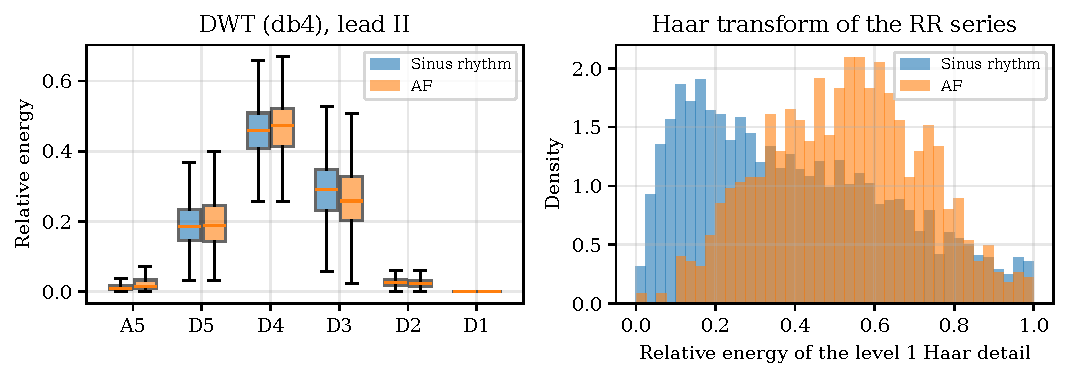
\includegraphics[width=\columnwidth]{wavelet_features.pdf}
\caption{Relative DWT subband energies of lead II (left) and relative energy of the level 1 Haar detail of the RR series (right), on 5000 public recordings.}
\label{fig:wav}
\end{figure}

\subsection{Radon Analysis}

Fig.~\ref{fig:radon} illustrates the mechanism of the Radon features. The recurrence plot of sinus rhythm shows blocks that repeat with the cardiac period and long diagonals, and its $45^\circ$ projection carries as much variance as the $0^\circ$ and $90^\circ$ projections. In AF the diagonals are short and irregularly spaced, and the $45^\circ$ peak falls well below the $0^\circ$ and $90^\circ$ peaks, which only reflect the block structure common to both classes. The feature distributions in Fig.~\ref{fig:radonf} confirm this behaviour at scale: in AF the variance ratio at $45^\circ$ is lower and the kurtosis of the $45^\circ$ projection is much higher, because a single peak (the main diagonal) remains instead of several. As reported in Table~\ref{tab:univ}, the kurtosis at $45^\circ$ is the most discriminative of all 172 features in both domains, above pNN50 and the Poincaré descriptors, and its discriminative power does not decrease when moving from public data to the ICU.

\begin{figure}[t]
\centering
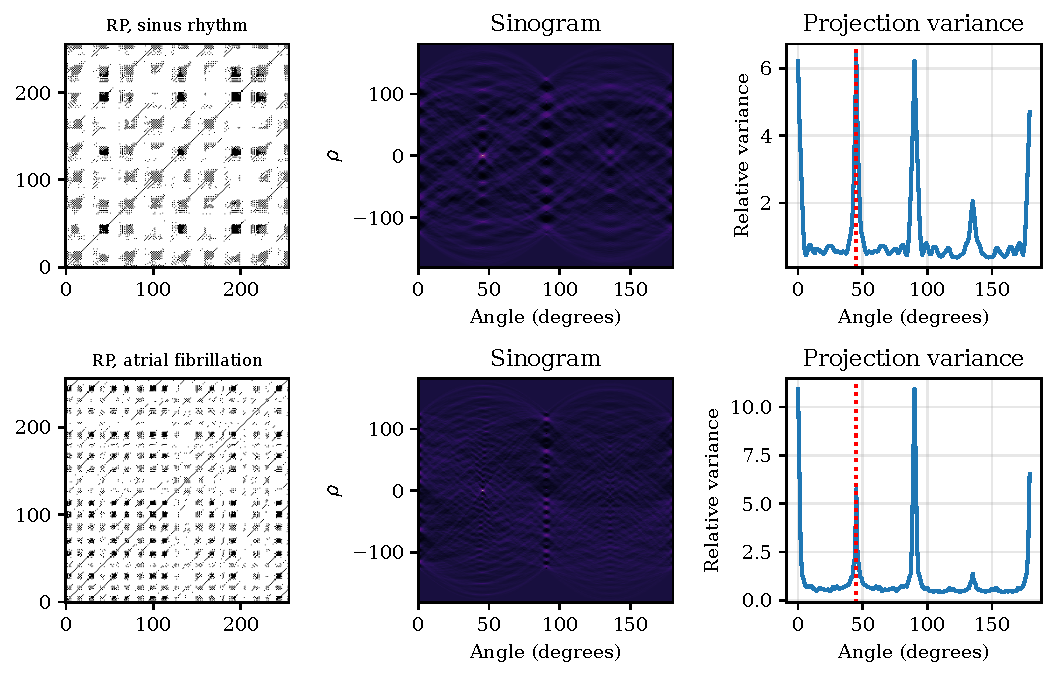
\includegraphics[width=\columnwidth]{radon.pdf}
\caption{Recurrence plot of lead II, its sinogram, and the variance of the Radon projection as a function of angle, for sinus rhythm (top) and AF (bottom). The dotted line marks $45^\circ$.}
\label{fig:radon}
\end{figure}

\begin{figure}[t]
\centering
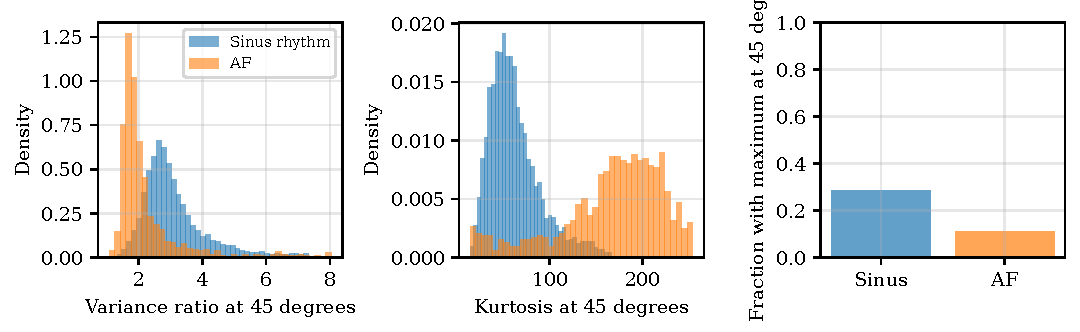
\includegraphics[width=\columnwidth]{radon_features.pdf}
\caption{Radon features of lead II on 5000 public recordings: variance ratio and kurtosis of the $45^\circ$ projection, and fraction of recordings whose maximum variance occurs at $45^\circ$.}
\label{fig:radonf}
\end{figure}

\begin{table}[t]
\centering
\caption{Univariate AUROC of selected features on the public data and on the 596 ICU recordings. For each feature the best lead is shown.}
\label{tab:univ}
\begin{tabular}{llcc}
\toprule
Group & Feature (lead) & Public & ICU \\
\midrule
Radon & Kurtosis at $45^\circ$ (V1) & 0.921 & 0.943 \\
Radon & Kurtosis at $45^\circ$ (II) & 0.918 & 0.946 \\
Base & pNN50 (V1) & 0.915 & 0.929 \\
Base & Shannon entropy (V1) & 0.903 & 0.930 \\
Base & SD1 accelerations (V1) & 0.904 & 0.922 \\
Base & P wave amplitude (I) & 0.874 & 0.678 \\
Base & P wave amplitude (II) & 0.873 & 0.820 \\
Spectral & Organization index (V1) & 0.804 & 0.692 \\
Wavelet & Haar RR detail level 1 (II) & 0.661 & 0.661 \\
Wavelet & DWT energy A5 (V1) & 0.650 & 0.552 \\
\bottomrule
\end{tabular}
\end{table}

\subsection{Spectral Analysis}

After QRST cancellation, the residual of V1 in sinus rhythm has its maximum at the lower edge of the band, where poorly cancelled T wave energy remains. In AF a clear mode appears between 5 and 8 Hz (Fig.~\ref{fig:spec}), equivalent to 300 to 480 atrial activations per minute, in agreement with the fibrillatory rates reported in the clinical literature~\cite{bollmann2006}; the median dominant frequency is 5.75 Hz in AF against 3.5 Hz in sinus rhythm. The spectral entropy is lower in AF. This seems to contradict the notion of disorder, but it reflects that the f waves concentrate power in one peak, while the sinus residual is close to white noise. The effect is strongest in V1, the lead closest to the atria.

\begin{figure}[t]
\centering
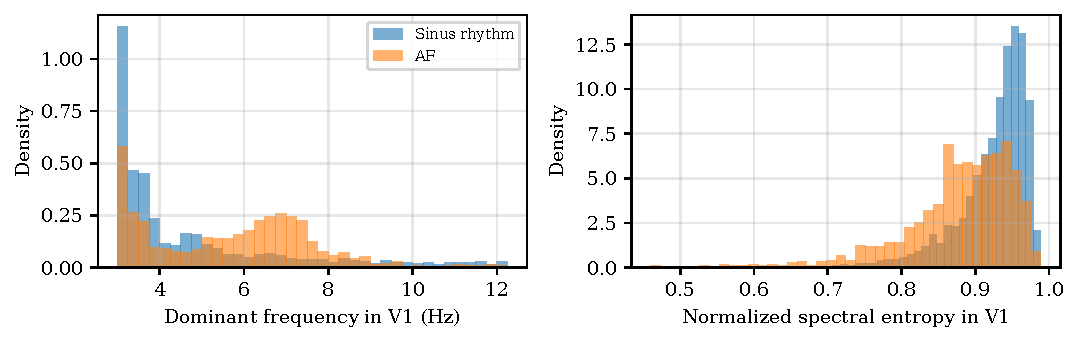
\includegraphics[width=\columnwidth]{spectral.pdf}
\caption{Dominant frequency and normalized spectral entropy of the atrial residual in V1, on 5000 public recordings.}
\label{fig:spec}
\end{figure}

\subsection{Cramér Rao Analysis}

Fig.~\ref{fig:crlb} and Table~\ref{tab:crlb} show that, up to a beat jitter of 20 ms, the variance of the least squares heart rate estimate coincides with the bound in~\eqref{eq:crlb}, with efficiencies between 0.96 and 1.06. At 40 ms the jitter becomes comparable to the QRS width, the detector starts to miss beats or to assign wrong beat indices, and the variance exceeds the bound by a factor of four, the threshold effect expected outside the small error regime. Even at 20 ms the standard deviation of the heart rate estimate is about 0.15 beats per minute. The mean heart rate of a 10 s window is therefore estimated almost without error, and the diagnostic information lies in the irregularity of the intervals, which is precisely what the HRV and Radon features measure.

\begin{figure}[t]
\centering
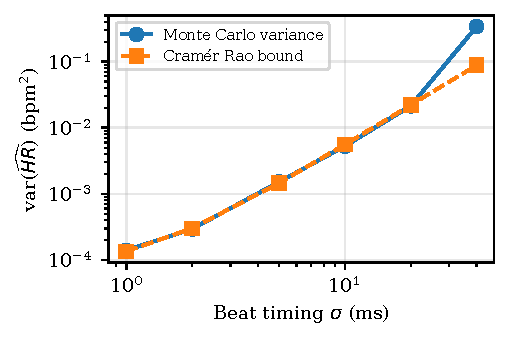
\includegraphics[width=0.7\columnwidth]{crlb.pdf}
\caption{Monte Carlo variance of the heart rate estimate and Cramér Rao bound as functions of the beat timing jitter, for synthetic 10 s ECGs at 73 beats per minute.}
\label{fig:crlb}
\end{figure}

\begin{table}[t]
\centering
\caption{Efficiency (bound divided by empirical variance) of the least squares heart rate estimator.}
\label{tab:crlb}
\begin{tabular}{lcccccc}
\toprule
$\sigma$ (ms) & 1 & 2 & 5 & 10 & 20 & 40 \\
\midrule
Efficiency & 0.96 & 1.02 & 0.96 & 1.06 & 1.03 & 0.26 \\
\bottomrule
\end{tabular}
\end{table}

\subsection{Ablation Study}

Fig.~\ref{fig:abl} reports F1 and AUROC with bootstrap intervals for the five feature sets. No extended set changes F1 significantly: the intervals overlap in every case and are about 0.15 wide, a direct consequence of the 49 positive cases. Within the ICU (configuration 2), the base features are already close to the ceiling and adding columns to 298 training samples changes little. Under domain shift (configuration 3), the full feature set raises the AUROC of CatBoost from 0.935 to 0.959 (paired difference 0.024, 95\% CI 0.004 to 0.050) and that of KNN from 0.907 to 0.932 (paired difference 0.026, 95\% CI 0.001 to 0.058), and the AUPRC of both models increases by 0.04 and 0.07, whereas LR, already at 0.97, does not improve (paired difference $-0.011$, 95\% CI $-0.036$ to 0.007). The paired intervals of the two nonlinear models exclude zero, although narrowly and without correction for the 24 comparisons of the study, so the nonlinear models recover a modest but consistent part of the gap that separated them from LR. Among the F1 differences, only two of the 24 paired intervals exclude zero (spectral features with LR in configuration 2 and Radon features with CatBoost in configuration 3), a number compatible with chance at this level of multiplicity.

\begin{figure}[t]
\centering
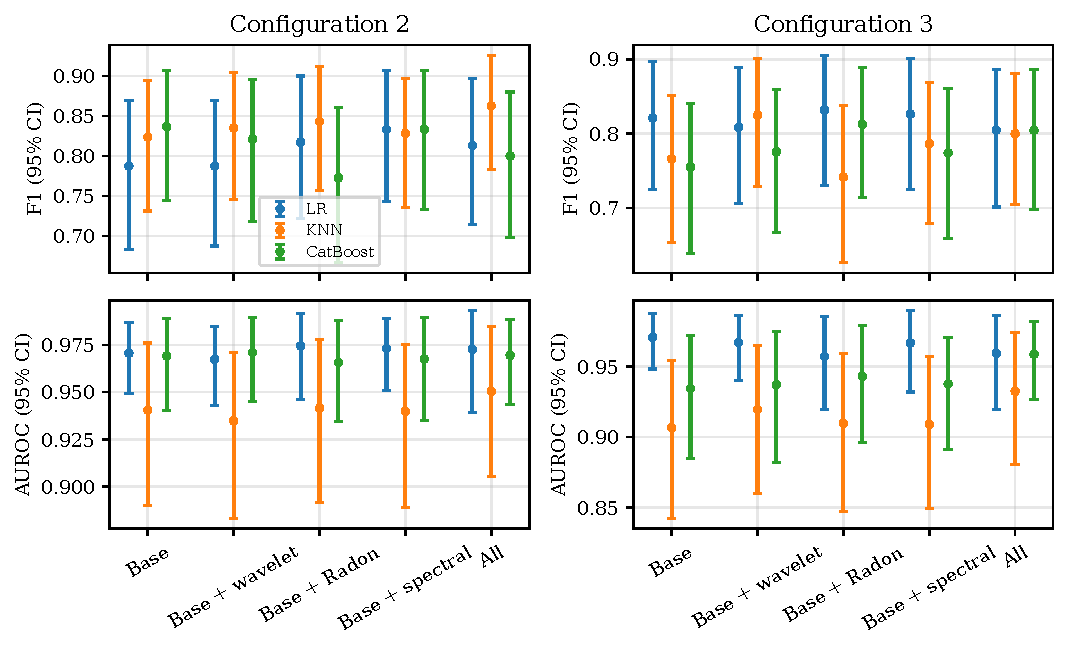
\includegraphics[width=\columnwidth]{ablation.pdf}
\caption{Ablation study. F1 (top) and AUROC (bottom) with 95\% bootstrap confidence intervals for LR, KNN, and CatBoost trained on five feature sets, in configuration 2 (left) and configuration 3 (right).}
\label{fig:abl}
\end{figure}

\subsection{Explanations}

Fig.~\ref{fig:shap} shows the global SHAP summary of the CatBoost model trained on public data with all features. The most influential features are not rhythm measures but the P wave amplitude of leads I and II: low amplitudes push the prediction strongly towards AF, which is the clinical criterion of absent P waves. They are followed by the dominant frequency, spectral entropy, and organization index of V1 and III, and by the Radon kurtosis of V1, all with the physiologically expected direction. The classical RR features rank lower individually because they are numerous and strongly correlated, and their attribution is shared among them. By group, the 27 base features per lead account for 57\% of the total mean absolute SHAP value, the spectral group for 18\%, the wavelet group for 13\%, and the Radon group for 12\%, even though the extended features are a minority of the columns.

\begin{figure}[t]
\centering
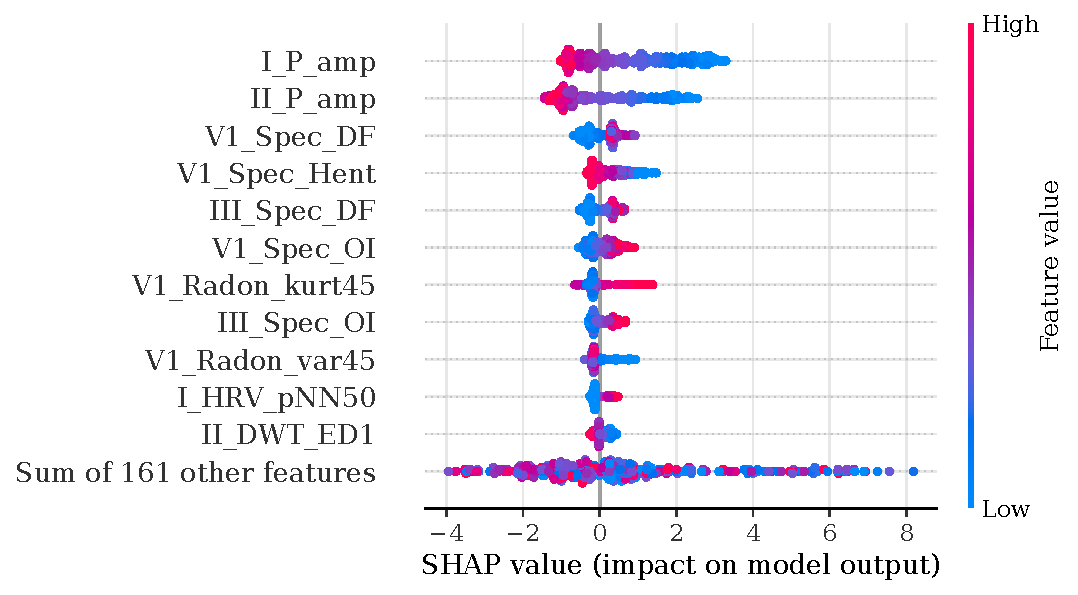
\includegraphics[width=\columnwidth]{shap_global.pdf}
\caption{SHAP summary of the CatBoost model of configuration 3 with all features, on the ICU test set. Each point is a recording, its color is the feature value, and its horizontal position is the contribution to the log odds of AF.}
\label{fig:shap}
\end{figure}

Fig.~\ref{fig:shaploc} explains the most confident error of each type. The false positive is a sinus rhythm with an almost absent P wave in lead I and highly variable RR intervals (high pNN50 and Shannon entropy), a profile compatible with sinus arrhythmia or frequent ectopic beats; the visible P wave in lead II and the absence of a fibrillatory peak in V1 push against AF but do not compensate. The false negative is the opposite case: an AF recording with apparent P waves in leads II and III and regular RR intervals (pNN50 equal to zero), which suggests atrial flutter with fixed conduction, grouped with AF in the dataset although its ventricular rhythm is regular.

\begin{figure}[t]
\centering
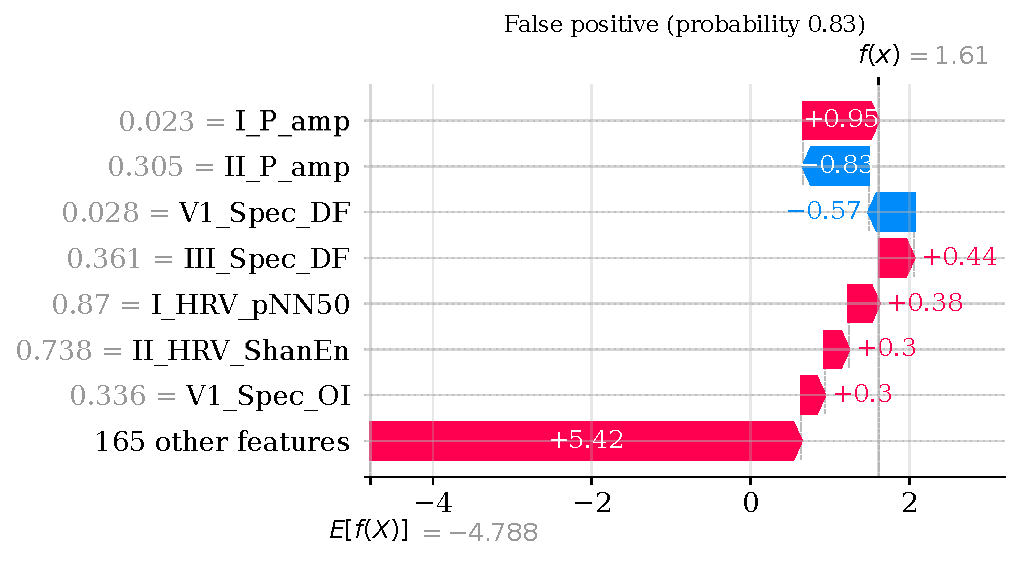
\includegraphics[width=\columnwidth]{shap_positive.pdf}\\[1mm]
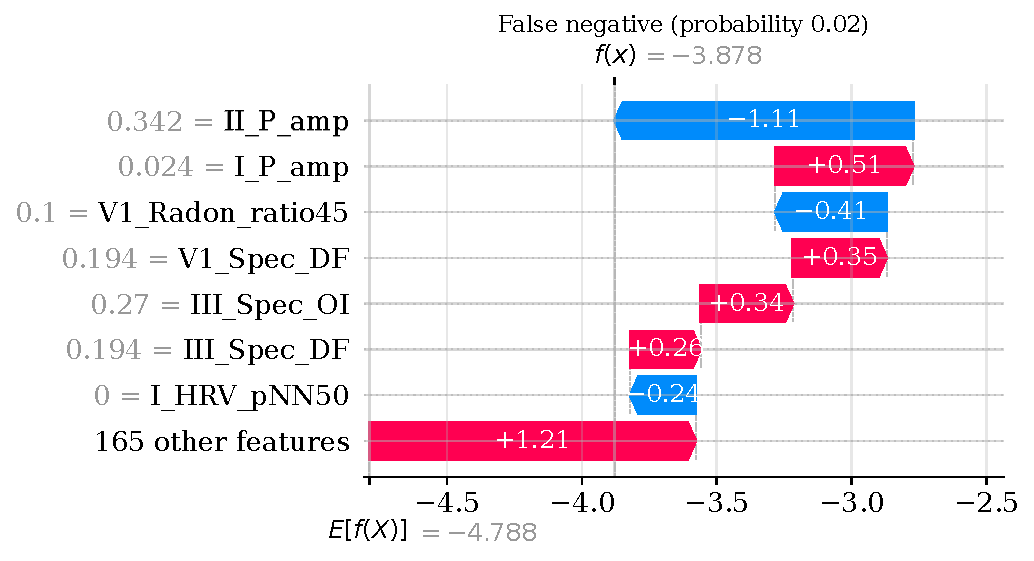
\includegraphics[width=\columnwidth]{shap_negative.pdf}
\caption{Local SHAP explanations of the most confident false positive (top) and false negative (bottom) of the model in Fig.~\ref{fig:shap}. Feature values are min max scaled.}
\label{fig:shaploc}
\end{figure}

\section{Discussion}
\label{sec:discussion}

\noindent\textbf{Reproducibility without code.} The feature based benchmark of~\cite{nassar2025} can be rebuilt from its text with deviations that are indistinguishable from the sampling noise of its test set. The residual differences have identifiable sources: random initialization (visible in the MLP), unspecified hyperparameters and missing value handling, NeuroKit2 settings for P wave delineation, small differences in the labeled public set (0.2\% fewer recordings), library versions, and the SVM subsample of configuration 3. None of them changes the ranking of the models or the conclusions. The width of the bootstrap intervals in Fig.~\ref{fig:abl} also shows that the single point estimates reported in the original tables cannot separate most models from each other.

\noindent\textbf{What the signal processing tools add.} The value of each tool depends on where it acts. The Radon transform of the recurrence plot condenses rhythm determinism into one number that is as discriminative as the best HRV measure and more stable across domains. The atrial spectrum adds information that the RR features cannot provide, namely the presence of organized f waves, and is the extended group that the model uses most. The discrete wavelet energies add little, not because the wavelet transform is unsuitable but because the reproduced 5 to 30 Hz filter removes the band where the f waves live; the scaleogram of the unfiltered lead shows that this information exists. The Cramér Rao analysis explains why heart rate itself is a weak feature: in 10 s it is estimated with a precision far finer than any clinical difference, so the classification must rely on irregularity and atrial morphology.

\noindent\textbf{Domain shift and the P wave.} The explanations offer a mechanism for the degradation observed in configuration 3. The P wave amplitude is the feature on which the tree model relies most, yet its univariate AUROC in lead I falls from 0.87 on public data to 0.68 on ICU data (Table~\ref{tab:univ}), plausibly because of the noisier baseline, the electrode placement, and the different lead configuration of bedside monitors. Rhythm features such as pNN50 and the Radon kurtosis, in contrast, keep their discriminative power in both domains. A model that leans on a feature whose meaning changes between domains will degrade, and this is consistent with the larger loss of the tree ensembles relative to LR and with the partial recovery of their AUROC when domain stable features are added.

\noindent\textbf{Limitations.} (1) The ICU test set contains only 49 AF episodes, so differences below about 0.05 in F1 cannot be resolved, and the AUROC gains of the extended features under domain shift, although their paired intervals exclude zero, are small and uncorrected for multiple comparisons. (2) Each configuration was trained once with a fixed seed. (3) The ICU data come from a single institution and the recordings last 10 s, which limits the estimation of spectral and recurrence features. (4) AF and atrial flutter share one label, and the explanations show that regular flutter is a source of false negatives. (5) Only the feature based part of~\cite{nassar2025} was reproduced; the convolutional and foundation models were not.

\section{Conclusion}
\label{sec:conclusion}

This work rebuilt the feature based AF detection benchmark of Nassar et al. for ICU electrocardiograms without access to the original code. The reproduced metrics of eight classifiers in two training configurations match the published ones within one or two misclassified episodes, and the main finding of the article, that logistic regression is the most robust model when training on public data and testing in the ICU, holds. Extending the feature set with signal processing tools from the course showed that their value depends on where they act: the Radon transform of the recurrence plot yields the single most discriminative and most domain stable feature, the atrial spectrum captures fibrillatory activity at the expected 5 to 8 Hz, the discrete wavelet energies add little after the 5 to 30 Hz filter, and the Cramér Rao bound confirms that the mean heart rate of a 10 s window carries little diagnostic information. SHAP explanations show that the models follow the clinical definition of AF and identify the P wave amplitude as the feature most affected by the shift to ICU data.

\noindent\textbf{Future work.} Four directions follow from these findings. The first is to evaluate the extended features with repeated cross validation or a larger ICU cohort to confirm the gains observed under domain shift. The second is to compute atrial features on a wider band, before the 5 to 30 Hz filter, so that the wavelet and spectral groups can access the full f wave content. The third is to separate atrial flutter from AF and to add flutter specific features such as the regularity of the atrial spectrum. The fourth is to make the P wave feature robust to ICU conditions, or to replace it by measures of atrial activity that transfer better between domains.

\section*{Code and Data Availability}

The code is available at
\begin{center}\small\url{https://github.com/ricardoamiel/Atrial-Fibrillation-Detection-in-Electrocardiograms}\end{center}
The repository contains the feature extraction and experiment scripts, the analysis notebook, and a resumable pipeline that downloads the public data, extracts the features, trains the models with checkpoints, and executes the notebook. The Kingston ICU AF dataset is available on PhysioNet under a credentialed data use agreement, and the PhysioNet/CinC 2021 data are openly available.

\begin{thebibliography}{99}
\bibitem{kornej2020} J. Kornej, C. S. Börschel, E. J. Benjamin, and R. B. Schnabel, ``Epidemiology of atrial fibrillation in the 21st century: novel methods and new insights,'' Circulation Research, vol. 127, no. 1, pp. 4 to 20, 2020.
\bibitem{moss2017} T. J. Moss et al., ``New onset atrial fibrillation in the critically ill,'' Critical Care Medicine, vol. 45, no. 5, pp. 790 to 797, 2017.
\bibitem{walkey2011} A. J. Walkey, R. S. Wiener, J. M. Ghobrial, L. H. Curtis, and E. J. Benjamin, ``Incident stroke and mortality associated with new onset atrial fibrillation in patients hospitalized with severe sepsis,'' JAMA, vol. 306, no. 20, pp. 2248 to 2254, 2011.
\bibitem{hindricks2021} G. Hindricks et al., ``2020 ESC guidelines for the diagnosis and management of atrial fibrillation,'' European Heart Journal, vol. 42, no. 5, pp. 373 to 498, 2021.
\bibitem{drew2014} B. J. Drew et al., ``Insights into the problem of alarm fatigue with physiologic monitor devices: a comprehensive observational study of consecutive intensive care unit patients,'' PLoS ONE, vol. 9, no. 10, e110274, 2014.
\bibitem{reyna2022} M. A. Reyna et al., ``Issues in the automated classification of multilead ECGs using heterogeneous labels and populations,'' Physiological Measurement, vol. 43, no. 8, 084001, 2022.
\bibitem{nassar2025} S. Nassar, N. Maghsoodi, S. Mannina, S. Addas, S. Sibley, G. Fichtinger, D. Pichora, D. Maslove, P. Abolmaesumi, and P. Mousavi, ``A dataset and benchmarks for atrial fibrillation detection from electrocardiograms of intensive care unit patients,'' arXiv:2512.18031, 2025.
\bibitem{pineau2021} J. Pineau et al., ``Improving reproducibility in machine learning research,'' Journal of Machine Learning Research, vol. 22, no. 164, pp. 1 to 20, 2021.
\bibitem{andreotti2017} F. Andreotti, O. Carr, M. A. F. Pimentel, A. Mahdi, and M. De Vos, ``Comparing feature based classifiers and convolutional neural networks to detect arrhythmia from short segments of ECG,'' in Proc. Computing in Cardiology, vol. 44, 2017.
\bibitem{jahan2022} M. S. Jahan et al., ``Short term atrial fibrillation detection using electrocardiograms: a comparison of machine learning approaches,'' International Journal of Medical Informatics, vol. 163, 104790, 2022.
\bibitem{clifford2017} G. D. Clifford et al., ``AF classification from a short single lead ECG recording: the PhysioNet/Computing in Cardiology Challenge 2017,'' in Proc. Computing in Cardiology, vol. 44, 2017.
\bibitem{makowski2021} D. Makowski et al., ``NeuroKit2: a Python toolbox for neurophysiological signal processing,'' Behavior Research Methods, vol. 53, pp. 1689 to 1696, 2021.
\bibitem{pan1985} J. Pan and W. J. Tompkins, ``A real time QRS detection algorithm,'' IEEE Transactions on Biomedical Engineering, vol. 32, no. 3, pp. 230 to 236, 1985.
\bibitem{sleepecg} C. Brunner et al., ``SleepECG: sleep stage detection using ECG,'' 2024. [Online]. Available: https://sleepecg.readthedocs.io
\bibitem{hannun2019} A. Y. Hannun et al., ``Cardiologist level arrhythmia detection and classification in ambulatory electrocardiograms using a deep neural network,'' Nature Medicine, vol. 25, no. 1, pp. 65 to 69, 2019.
\bibitem{ribeiro2020} A. H. Ribeiro et al., ``Automatic diagnosis of the 12 lead ECG using a deep neural network,'' Nature Communications, vol. 11, 1760, 2020.
\bibitem{mckeen2025} K. McKeen et al., ``ECG FM: an open electrocardiogram foundation model,'' JAMIA Open, vol. 8, no. 5, ooaf122, 2025.
\bibitem{li2025} J. Li et al., ``An electrocardiogram foundation model built on over 10 million recordings,'' NEJM AI, vol. 2, no. 7, 2025.
\bibitem{addison2005} P. S. Addison, ``Wavelet transforms and the ECG: a review,'' Physiological Measurement, vol. 26, no. 5, pp. R155 to R199, 2005.
\bibitem{mallat2009} S. Mallat, A Wavelet Tour of Signal Processing: The Sparse Way, 3rd ed. Burlington, MA, USA: Academic Press, 2009.
\bibitem{takens1981} F. Takens, ``Detecting strange attractors in turbulence,'' in Dynamical Systems and Turbulence, Lecture Notes in Mathematics, vol. 898. Berlin, Germany: Springer, 1981, pp. 366 to 381.
\bibitem{marwan2007} N. Marwan, M. C. Romano, M. Thiel, and J. Kurths, ``Recurrence plots for the analysis of complex systems,'' Physics Reports, vol. 438, no. 5, pp. 237 to 329, 2007.
\bibitem{deans1983} S. R. Deans, The Radon Transform and Some of Its Applications. New York, NY, USA: Wiley, 1983.
\bibitem{stridh2001} M. Stridh and L. Sörnmo, ``Spatiotemporal QRST cancellation techniques for analysis of atrial fibrillation,'' IEEE Transactions on Biomedical Engineering, vol. 48, no. 1, pp. 105 to 111, 2001.
\bibitem{bollmann2006} A. Bollmann, D. Husser, L. Mainardi, F. Lombardi, P. Langley, A. Murray, J. J. Rieta, J. Millet, S. B. Olsson, M. Stridh, and L. Sörnmo, ``Analysis of surface electrocardiograms in atrial fibrillation: techniques, research, and clinical applications,'' Europace, vol. 8, no. 11, pp. 911 to 926, 2006.
\bibitem{lundberg2017} S. M. Lundberg and S. I. Lee, ``A unified approach to interpreting model predictions,'' in Advances in Neural Information Processing Systems, vol. 30, 2017.
\bibitem{lundberg2020} S. M. Lundberg et al., ``From local explanations to global understanding with explainable AI for trees,'' Nature Machine Intelligence, vol. 2, no. 1, pp. 56 to 67, 2020.
\bibitem{reyna2021} M. A. Reyna et al., ``Will two do? Varying dimensions in electrocardiography: the PhysioNet/Computing in Cardiology Challenge 2021,'' in Proc. Computing in Cardiology, vol. 48, 2021.
\bibitem{goldberger2000} A. L. Goldberger et al., ``PhysioBank, PhysioToolkit, and PhysioNet: components of a new research resource for complex physiologic signals,'' Circulation, vol. 101, no. 23, pp. e215 to e220, 2000.
\bibitem{ke2017} G. Ke et al., ``LightGBM: a highly efficient gradient boosting decision tree,'' in Advances in Neural Information Processing Systems, vol. 30, 2017.
\bibitem{chen2016} T. Chen and C. Guestrin, ``XGBoost: a scalable tree boosting system,'' in Proc. ACM SIGKDD Int. Conf. Knowledge Discovery and Data Mining, 2016, pp. 785 to 794.
\bibitem{prokhorenkova2018} L. Prokhorenkova, G. Gusev, A. Vorobev, A. V. Dorogush, and A. Gulin, ``CatBoost: unbiased boosting with categorical features,'' in Advances in Neural Information Processing Systems, vol. 31, 2018.
\bibitem{kay1993} S. M. Kay, Fundamentals of Statistical Signal Processing: Estimation Theory. Upper Saddle River, NJ, USA: Prentice Hall, 1993.
\bibitem{efron1993} B. Efron and R. J. Tibshirani, An Introduction to the Bootstrap. New York, NY, USA: Chapman and Hall, 1993.
\end{thebibliography}

\end{document}
